\documentclass[a4paper,12pt]{article} 

%%% Работа с русским языком
\usepackage{cmap}					% поиск в PDF
\usepackage{mathtext} 				% русские буквы в фомулах
\usepackage[T2A]{fontenc}			% кодировка
\usepackage[utf8]{inputenc}			% кодировка исходного текста
\usepackage[english,russian]{babel}	% локализация и переносы

%%% Дополнительная работа с математикой
\usepackage{amsmath,amsfonts,amssymb,amsthm,mathtools, gensymb} % AMS
\usepackage{icomma} % "Умная" запятая: $0,2$    ф--- число, $0, 2$ --- перечисление

%%Таблица
\usepackage[table,xcdraw]{xcolor}
\usepackage{caption}
\usepackage{floatrow}
\floatsetup[table]{capposition=top}
\floatsetup[wrapfigure]{capposition=bottom}
\usepackage{multirow}

\usepackage{hyperref}

%Отступы и поля 
\textwidth=18cm
\oddsidemargin=-1cm
\topmargin=-2cm
\textheight=25cm


%% Номера формул
\mathtoolsset{showonlyrefs=false} % Показывать номера только у тех формул, на которые есть \ref{} в тексте.

%% Шрифты
\usepackage{euscript}	 % Шрифт Евклид
\usepackage{mathrsfs} % Красивый матшрифт

%% Свои команды
\DeclareMathOperator{\sgn}{\mathop{sgn}}

%% Перенос знаков в формулах (по Львовскому)
\newcommand*{\hm}[1]{#1\nobreak\discretionary{}
{\hbox{$\mathsurround=0pt #1$}}{}}

%% Стиль страницы
\usepackage{fancyhdr}

%% Для рисунков
\usepackage{graphicx}
\usepackage[export]{adjustbox}
\usepackage{float}
\usepackage{ragged2e}
\usepackage{wrapfig}

\pagestyle{fancy}
\begin{document}
\begin{titlepage}
\begin{center}
%\vspace*{1cm}
\large{\small ФЕДЕРАЛЬНОЕ ГОСУДАРСТВЕННОЕ АВТОНОМНОЕ ОБРАЗОВАТЕЛЬНОЕ\\ УЧРЕЖДЕНИЕ ВЫСШЕГО ОБРАЗОВАНИЯ \\ МОСКОВСКИЙ ФИЗИКО-ТЕХНИЧЕСКИЙ ИНСТИТУТ\\ (НАЦИОНАЛЬНЫЙ ИССЛЕДОВАТЕЛЬСКИЙ УНИВЕРСИТЕТ)\\ ФАКУЛЬТЕТ АЭРОКОСМИЧЕСКИХ ТЕХНОЛОГИЙ}
\vfill
\line(1,0){490}\\[1mm]
\huge{Лабораторная работа 5.1}\\
\huge\textbf{Измерение коэффициента ослабления потока $\gamma$-лучей в веществе и определение их энергии}\\
\line(1,0){490}\\[1mm]
\vfill
\begin{flushright}
\normalsize{Рогозин Владимир}\\
\normalsize{\textbf{Группа Б03-106}}\\
\end{flushright}
\end{center}
\end{titlepage}
\fancyhead[L] {Работа 5.1}

\textbf{Цель работы}:
С помощью сцинтилляционного счетчика измеряются линейные коэффициенты ослабления потока $\gamma$-лучей в свинце, железе и алюминии; по их величине определяется энергия $\gamma$-квантов.


% \textbf{Оборудование}:
% лазер; кассета с набором сеток разного
% периода; линзы; щель с микрометрическим винтом; оптический стол
% c набором рейтеров и крепёжных винтов; экран; линейка.


\section{Теоретические сведения}
Гамма-лучи возникают при переходе возбужденных ядер из одного энергетического состояния в другое, более низкое. Энергия $\gamma$-квантов обычно заключена между несколькими десятками килоэлектрон-вольт и несколькими миллионами электрон-вольт. Гамма-кванты не несут электрического заряда, их масса равна нулю. Проходя через вещество, пучок $\gamma$-квантов постепенно ослабляется. Ослабление происходит по экспоненциальному закону, который может быть записан в двух эквивалентных формах:
\begin{equation}\label{eq: Intensity dying 1}
    I = I_0e^{-\mu l}
\end{equation}
\begin{equation}\label{eq: Intensity dying 2}
    I = I_0e^{-\mu' m_1}
\end{equation}
В этих формулах $I$, $I_0$ -- интенсивности прошедшего и падающего излучений, $l$ -- длина пути, пройденного пучком $\gamma$-лучей, $m_1$ -- масса пройденного вещества, приходящаяся на единицу площади, $\mu$ и $\mu'$ -- константы, величина которых зависит от вещества, сквозь которое проходят $\gamma$-лучи.

Ослабление потока $\gamma$-лучей, происходящее при прохождении среды, связано с тремя эффектами: фотоэлектрическим поглощением, комптоновским рассеянием и с генерацией электрон-позитронных пар.

\subsection{Фотоэлектрическое поглощение}
При столкновении $\gamma$-квантов с электронами внутренних атомных оболочек может происходить поглощение квантов. Энергия $\gamma$-кванта передается соответствующему электрону, а импульс делится между этим электроном и оставшимся после его вылета ионом. Свободный электрон не может поглотить $\gamma$-квант, так как при этом невозможно одновременно удовлетворить законам сохранения энергии и импульса. Наружные электроны не принимают участия в фотоэлектрическом поглощении, потому что они слабо связаны в атоме, так что их практически можно считать свободными. Вероятность $dP_\text{ф}$ фотоэлектрического поглощения $\gamma$-квантов пропорциональна длине пути $dl$ и плотности электронов (на внутренних оболочках атомов) в среде:
\begin{equation}\label{eq: Photoelectric effect differential probability}
    dP_\text{ф} = \sigma_\text{ф}n_1dl,
\end{equation}
где $n_1$ -- плотность внутренних электронов, а $\sigma_\text{ф}$ -- поперечное сечение фотоэлектрического поглощения. Поперечное сечение характеризует вероятность фотоэффекта, рассчитанную на один электрон.

Связь между коэффициентом поглощения для фотоэффекта $\mu_\text{ф}$ , входящим в формулу \ref{eq: Intensity dying 1}, и сечением $\sigma_\text{ф}$ находится как
\begin{equation}\label{eq: Intensity dying coeff}
    \mu_\text{ф} = \sigma_\text{ф}n_1.
\end{equation}

Пусть в результате фотоэффекта энергия $\gamma$-кванта передается электрону, находящемуся на $i$-ой оболочке атома. Пусть $W_i$ энергия связи этого электрона. После вылета из атома электрон приобретает кинетическую энергию
\begin{equation}\label{eq: Electron kinetic energy}
    T_i = \hbar\omega - W_i.
\end{equation}

Освободившееся после вылета электрона место заполняется затем одним из электронов с вышележащих оболочек.

Вероятность фотоэффекта сложным образом зависит от энергии $\gamma$-лучей и от заряда ядер. Для оценок можно пользоваться формулой
\begin{equation}\label{eq: Photoelectric effect probability}
    \sigma_\text{ф} \propto \frac{Z^5}{(\hbar\omega)^{3,5}}.
\end{equation}

Из формулы \ref{eq: Photoelectric effect probability} видно, что вероятность фотоэффекта быстро возрастает при переходе от легких к тяжелым элементам и резко падает с увеличением энергии $\gamma$-квантов.

\subsection{Комптоновское рассеяние}
Комптоновским рассеянием называется упругое столкновение $\gamma$-кванта с электроном. При таком столкновении $\gamma$-квант передает электрону часть своей энергии, величина которой определяется углом рассеяния. В отличие от фотоэффекта, который может идти только на сильно связанных электронах, комптоновское рассеяние происходит на свободных или слабосвязанных электронах. Роль эффекта Комптона становится существенной только тогда, когда энергия квантов становится много больше энергии связи электронов в атоме. Атомные электроны в этом случае можно считать практически свободными.

Вероятность комптон-эффекта сложным образом зависит от энергии $\gamma$-квантов. В том случае, когда энергия $\gamma$-кванта много больше энергии покоя электрона, формула сильно упрощается, и выражение для сечения комптон-эффекта приобретает простой вид:
\begin{equation}\label{eq: Compton effect probability}
    \sigma_K = \pi r^2\frac{mc^2}{\hbar\omega}\left(\ln\frac{2\hbar\omega}{mc^2} + \frac{1}{2}\right),
\end{equation}
где $r \approx 2,8 \cdot 10^{-13}$ см -- классический радиус электрона, а $m$ -- его масса. Из формулы \ref{eq: Compton effect probability} следует, что сечение комптон-эффекта с ростом энергии фотонов падает далеко не так резко, как сечение фотоэффекта.

Сечение $\sigma_K$ относится к одному свободному электрону, в то время как приведенное выше сечение фотоэффекта рассчитано на атом. Комптоновское рассеяние, отнесенное к атому, оказывается в $Z$ раз больше.

Комптоновский коэффициент линейного ослабления $\mu_K$ связан с сечением $\sigma_K$ формулой, аналогичной \ref{eq: Intensity dying coeff}. Под $n$ следует в этом случае понимать плотность слабо связанных электронов, т. е. практически полную плотность электронов в веществе.

\subsection{Образование пар}
При энергиях $\gamma$-лучей, превышающих $2mc^2 = 1,02$ МэВ, становится возможен процесс поглощения $\gamma$-лучей, связанный с образованием электрон-позитронных пар. Рождение пар не может происходить в вакууме, оно возникает в электрическом поле ядер. Вероятность этого процесса приблизительно пропорциональна $Z^2$ и сложным образом зависит от энергии фотона. При энергиях больше $2mc^2$ фотоэффект даже для самых тяжелых ядер уже не играет практически никакой роли. Вероятность образования пар должна поэтому сравниваться с вероятностью комптоновского рассеяния. При энергиях, с которыми
приходится иметь дело при изучении ядер, рождение пар существенно только в самых тяжелых элементах.

\subsection{Полный коэффициент ослабления потока $\gamma$-лучей.}
Полный линейный коэффициент $\mu$ ослабления пучка $\gamma$-квантов при прохождении через вещество равен сумме коэффициентов для всех трех рассмотренных процессов.

В \textit{хорошей геометрии} опыта, т. е. в условиях, когда исследуется прохождение сквозь вещество узкого параллельного пучка $\gamma$-лучей, не только фотоэлектрическое поглощение и генерация пар, но и комптоновское рассеяние выводит $\gamma$-кванты из пучка. Поэтому при прохождении через вещество меняется только количество, но не энергия $\gamma$-квантов в пучке, так что коэффициент $\mu$, характеризующий поглощение $\gamma$-квантов в веществе, не зависит от длины пути. Обозначим через $-dN$ число $\gamma$-квантов, выбывших из пучка на пути $dl$. Это число пропорционально имеющемуся их числу $N$ и пройденному пути $dl$. Имеем, следовательно,
\begin{equation}\label{eq: Quitting photons}
    -dN = \mu Ndl.
\end{equation}
Интегрируя уравнение \ref{eq: Quitting photons} от нулевой толщины до заданной, получим формулу \ref{eq: Intensity dying 1}:
\begin{equation}\label{eq: Number of photons dying}
    N = N_0e^{-\mu l}.
\end{equation}

В \textit{плохой геометрии}, когда рассеянные под небольшими углами $\gamma$-кванты остаются в пучке, их спектр с прохождением вещества меняется, и формула \ref{eq: Intensity dying 1}, вообще говоря, неприменима. Эта формула, однако, работает и в этом случае лучше, чем можно было бы ожидать.
Причина хорошего согласия заключается в том, что $\gamma$-кванты с энергией $1-2$ МэВ, потерявшие энергию из-за комптоновского рассеяния, быстро выбывают из пучка из-за резкого увеличения сечений $\sigma_\text{ф}$ и $\sigma_K$.

В данной работе коэффициент ослабления $\mu$ измеряется в хорошей геометрии. Из формулы \ref{eq: Intensity dying 1} имеем
\begin{equation}\label{eq: Attenuation coefficient}
    \mu = \frac{1}{l}\ln\frac{N_0}{N}.
\end{equation}
Для определения коэффициента ослабления нужно, таким образом, измерить толщину образца $l$, число падающих частиц $N_0$ и число частиц $N$, прошедших через образец.

\section{Экспериментальная установка}
    Схема установки, используемой в работе, показана на рис. \hyperref[fig: Exp setup]{1}. Свинцовый коллиматор выделяет узкий почти параллельный пучок $\gamma$-квантов, проходящий через набор поглотителей П и регистрируемый сцинтилляционным счетчиком. Сигналы от счетчика усиливаются и регистрируются пересчетным прибором ПП. Высоковольтный выпрямитель ВВ обеспечивает питание сцинтилляционного счетчика.
    \begin{figure}[H]\label{fig: Exp setup}
        \centering
        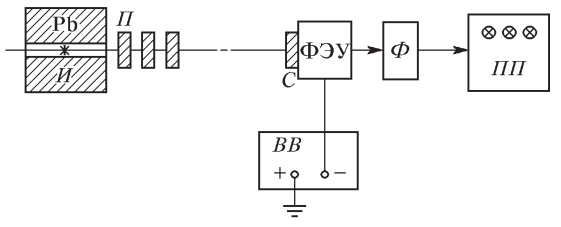
\includegraphics[width = 0.8\textwidth]{Exp setup.png}
        \caption{Блок-схема установки, используемой для измерения коэффициентов ослабления потока $\gamma$-лучей: И -- источник $\gamma$-лучей; Pb -- свинцовый контейнер с коллиматорным каналом; П -- набор поглотителей; С -- сцинтиллятор -- кристалл NaI(Tl); -- формирователь-выпрямитель}
    \end{figure}
    
    \begin{figure}[H]\label{fig: Scattering scheme}
        \centering
        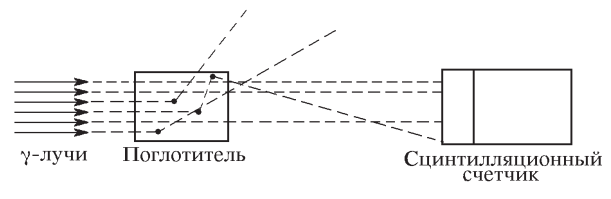
\includegraphics[width = 0.8\textwidth]{Scattering scheme.png}
        \caption{Схема рассеяния $\gamma$-квантов в поглотителе}
    \end{figure}

    При недостаточно хорошей геометрии в результаты опытов могут вкрасться существенные погрешности. В реальных установках всегда имеется конечная вероятность того, что $\gamma$-квант провзаимодействует в поглотителе несколько раз до того, как попадет в детектор. Чтобы уменьшить число таких случаев, в данной работе сцинтилляционный счетчик расположен на большом расстоянии от источника $\gamma$-квантов, а поглотители имеют небольшие размеры. Их следует устанавливать за коллиматорной щелью на некотором расстоянии друг от друга, чтобы испытавшие комптоновское рассеяние и выбывшие из прямого потока кванты с меньшей вероятностью могли в него вернуться.

\section{Обработка данных}
Включим пересчетный прибор и высоковольтный выпрямитель, дадим им прогреться в течение 5-10 минут.

\subsection{Проверка работоспособности установки}
\begin{enumerate}
    \item
    Убедимся в том, что установка «чувствует» $\gamma$-лучи. Для этого подадим на ФЭУ напряжение, указанное на установке $V = 1,5$ В. Измерим скорость
    счета при полностью открытом коллиматоре, а затем при коллиматоре, закрытом свинцовой пробкой. Результаты занесём в таблицу.

    \begin{table}[H]\label{tab: N in two regimes}
        \begin{tabular}{|
            >{\columncolor[HTML]{FFFFFF}}c |
            >{\columncolor[HTML]{FFFFFF}}c |
            >{\columncolor[HTML]{FFFFFF}}c |}
            \hline
            {\color[HTML]{000000} }                    & {\color[HTML]{000000} {$t$, c}} & {\color[HTML]{000000} {$N$, частиц}} \\ \hline
            {\color[HTML]{000000} Открытый коллиматор} & {\color[HTML]{000000} 10}              & {\color[HTML]{000000} 275328}               \\ \hline
            {\color[HTML]{000000} Закрытый коллиматор} & {\color[HTML]{000000} 10}              & {\color[HTML]{000000} 412}                  \\ \hline
        \end{tabular}
        \caption{Количество зарегистрированных частиц за время наблюдения }
    \end{table}
    По результатам измерений видно, что скорость счёта частиц резко уменьшилась, как это и должно быть, а значит установка работает корректно. 
    
\end{enumerate}

\subsection{Измерение фона}
При любом измерении присутствует постоянный фон, обусловленный шумом ФЭУ и посторонними частицами: космическим излучением, $\gamma$-квантами от соседних источников, квантами, рассеянными на стенах комнаты и в стенках прибора, и т. д.
\begin{enumerate}
    \item
    Для определения фона закроем коллиматор толстой свинцовой пробкой и будем измерять количество частиц в таком режиме. Оставшийся счет не связан, очевидно, с квантами, летящими в пучке. Результат измерений приведён в таблице ниже. 
    \begin{table}[H]\label{tab: N noise}
        \begin{tabular}{|
            >{\columncolor[HTML]{FFFFFF}}c |
            >{\columncolor[HTML]{FFFFFF}}c |
            >{\columncolor[HTML]{FFFFFF}}c |}
            \hline
            {\color[HTML]{000000} }    & {\color[HTML]{000000} $t$, с} & {\color[HTML]{000000} $N$, частиц} \\ \hline
            {\color[HTML]{000000} Фон} & {\color[HTML]{000000} 240}    & {\color[HTML]{000000} 10100}       \\ \hline
        \end{tabular}
        \caption{Количество фоновых частиц за время наблюдения}
    \end{table}
\end{enumerate}

\subsection{Исследование поглощения $\gamma$-лучей в свинце, железе и алюминии}
\begin{enumerate}
    \item
    Теперь будем измерять количество зарегистрированных частиц в зависимости от толщины барьера (материала). 
    \begin{table}[H]\label{tab: N result}
        \begin{tabular}{|
            >{\columncolor[HTML]{FFFFFF}}c |
            >{\columncolor[HTML]{FFFFFF}}c |
            >{\columncolor[HTML]{FFFFFF}}c |
            >{\columncolor[HTML]{FFFFFF}}c |}
            \hline
            {\color[HTML]{000000} Материал} &
              \cellcolor[HTML]{FFFFFF}{\color[HTML]{000000} $d$, мм} &
              \cellcolor[HTML]{FFFFFF}{\color[HTML]{000000} $t$, с} &
              {\color[HTML]{000000} $N$, частиц} \\ \hline
            \cellcolor[HTML]{FFFFFF}{\color[HTML]{000000} } &
              \cellcolor[HTML]{FFFFFF}{\color[HTML]{000000} $4,8 \pm 0,2$} &
              \cellcolor[HTML]{FFFFFF}{\color[HTML]{000000} $60$} &
              {\color[HTML]{000000} $973830$} \\ \cline{2-4} 
            \cellcolor[HTML]{FFFFFF}{\color[HTML]{000000} } &
              {\color[HTML]{000000} $9,3 \pm 0,4$} &
              {\color[HTML]{000000} $60$} &
              {\color[HTML]{000000} $595580$} \\ \cline{2-4} 
            \multirow{-3}{*}{\cellcolor[HTML]{FFFFFF}{\color[HTML]{000000} Свинец}} &
              {\color[HTML]{000000} $13,8 \pm 0,6$} &
              {\color[HTML]{000000} $60$} &
              {\color[HTML]{000000} $367044$} \\ \hline
            \cellcolor[HTML]{FFFFFF}{\color[HTML]{000000} } &
              \cellcolor[HTML]{FFFFFF}{\color[HTML]{000000} $19,7 \pm 0,2$} &
              {\color[HTML]{000000} $30$} &
              {\color[HTML]{000000} $572233$} \\ \cline{2-4} 
            \cellcolor[HTML]{FFFFFF}{\color[HTML]{000000} } &
              {\color[HTML]{000000} $39,7 \pm 0,4$} &
              {\color[HTML]{000000} $30$} &
              {\color[HTML]{000000} $379393$} \\ \cline{2-4} 
            \multirow{-3}{*}{\cellcolor[HTML]{FFFFFF}{\color[HTML]{000000} Алюмииний}} &
              {\color[HTML]{000000} $59,7 \pm 0,6$} &
              {\color[HTML]{000000} $30$} &
              {\color[HTML]{000000} $250502$} \\ \hline
            \cellcolor[HTML]{FFFFFF}{\color[HTML]{000000} } &
              {\color[HTML]{000000} $10,2 \pm 0,2$} &
              {\color[HTML]{000000} $40$} &
              {\color[HTML]{000000} $658289$} \\ \cline{2-4} 
            \cellcolor[HTML]{FFFFFF}{\color[HTML]{000000} } &
              {\color[HTML]{000000} $20,2 \pm 0,4$} &
              {\color[HTML]{000000} $40$} &
              {\color[HTML]{000000} $373012$} \\ \cline{2-4} 
            \multirow{-3}{*}{\cellcolor[HTML]{FFFFFF}{\color[HTML]{000000} Железо}} &
              {\color[HTML]{000000} $30,3 \pm 0,6$} &
              {\color[HTML]{000000} $40$} &
              {\color[HTML]{000000} $211438$} \\ \hline
        \end{tabular}
        \caption{Результаты измерений количества прошедших частиц для различных материалов}
    \end{table}
    Погрешность измерения длины образца с помощью штангенциркуля равна $\sigma_l = 0,2$ мм.
    \item 
    По данным из таблицы построим график зависимости длины пути $l$ от логарифма зарегистрированных частиц $\ln(N)$. Относительная погрешность числа частиц $N$ вычислялась по формуле \fbox{$\varepsilon_N \approx \frac{1}{\sqrt{N}}$}.    
    \item 
    Занесём в таблицу результаты определения коэффициента ослабления для каждого из материалов.
    \begin{table}[H]\label{tab: mu results}
        \centering
        \begin{tabular}{|
            >{\columncolor[HTML]{FFFFFF}}c |
            >{\columncolor[HTML]{FFFFFF}}c |
            >{\columncolor[HTML]{FFFFFF}}c |
            >{\columncolor[HTML]{FFFFFF}}c |}
            \hline
            {\color[HTML]{000000} Материал}                & {\color[HTML]{000000} Pb}   & {\color[HTML]{000000} Al}   & {\color[HTML]{000000} Fe}   \\ \hline
            {\color[HTML]{000000} $\mu$,$\text{ см}^{-1}$} & {\color[HTML]{000000} 1,09} & {\color[HTML]{000000} 0,21} & {\color[HTML]{000000} 0,57} \\ \hline
            {\color[HTML]{000000} $\varepsilon_\mu$, $\%$} & {\color[HTML]{000000} 0,1}  & {\color[HTML]{000000} 0,4}  & {\color[HTML]{000000} 0,6}  \\ \hline
        \end{tabular}
        \caption{Результаты определения коэффициента ослабления}
    \end{table}  
\end{enumerate}

\subsection{Определение средней энергии испускаемых $\gamma$-лучей}
\begin{enumerate}
    \item 
    Используя известные значения коэффициентов поглощения для Pb, Al и Fe.
    \item 
    В таблице коэффициентам со значениями $1,01$ $\text{см}^{-1}$ $0,21$ $\text{см}^{-1}$, $0,563$ $\text{см}^{-1}$ для Pb, Al, Fe соответствуют значения энергии $\gamma$-кванта $0,8$ МэВ, $0,6$ МэВ, $0,7$ МэВ соответственно. Отсюда мы можем сделать вывод, что энергия $\gamma$-излучения с хорошей точностью лежит в диапазоне $0,6-0,8$ МэВ.
\end{enumerate}

\subsection{Измерение уровня радиации}
\begin{enumerate}
    \item
    Дозиметром измерим уровень радиации в различных местах помещения, результаты занесём в таблицу.
    \begin{table}[H]\label{tab: radiation results}
        \centering
        \begin{tabular}{|
            >{\columncolor[HTML]{FFFFFF}}c |
            >{\columncolor[HTML]{FFFFFF}}c |}
            \hline
            {\color[HTML]{000000} Место}                        & {\color[HTML]{000000} Уровень радиации, мкЗв/ч} \\ \hline
            {\color[HTML]{000000} 1 этаж ЛК}                    & {\color[HTML]{000000} 0,13}                     \\ \hline
            {\color[HTML]{000000} Рабочее место в лаборатории}  & {\color[HTML]{000000} 0,17}                     \\ \hline
            {\color[HTML]{000000} Свинцовая оболочка установки} & {\color[HTML]{000000} 0,16}                     \\ \hline
            {\color[HTML]{000000} Непосредственно излучение} & {\color[HTML]{000000} \textgreater 9,99} \\ \hline
        \end{tabular}
        \caption{Результаты измерения радиации }
    \end{table}
    Безопасным считается уровень радиации до величины, приблизительно $0,5$ микрозиверт в час, таким образом можем сделать вывод, что в лаборатории вне непосредственного контакта 
    с пучком $\gamma$-квантов уровень радиации является допустимым. Свинцовая оболочка установки защищает от избыточной радиации, что делает возможным нахождение в лаборатории и работу на установке.
\end{enumerate}

\section{Вывод}
В данной работе изучалось поглощение $\gamma$-лучей в свинце, железе и алюминии, а также измерялся радиационный фон в помещении. В результате удалось:
\begin{itemize}
    \item
    определить коэффициент поглощения для свинца $\mu_{Pb} = 1,09 \text{ см}^{-1}$ , железа $\mu_{Fe} = 0,57 \text{ см}^{-1}$ и алюминия $\mu_{Al} = 0,21 \text{ см}^{-1}$
    
    \item
    дозиметром измерить радиационный фон в различных помещениях корпуса, убедиться, что радиационнный фон является допустимым по норме 
    
\end{itemize}

\newpage
%%%%%%%%%%%%%%%%%%%%%%%%% Графики
\begin{figure}[H]\label{fig: l(lnN)Pb}
    \centering
    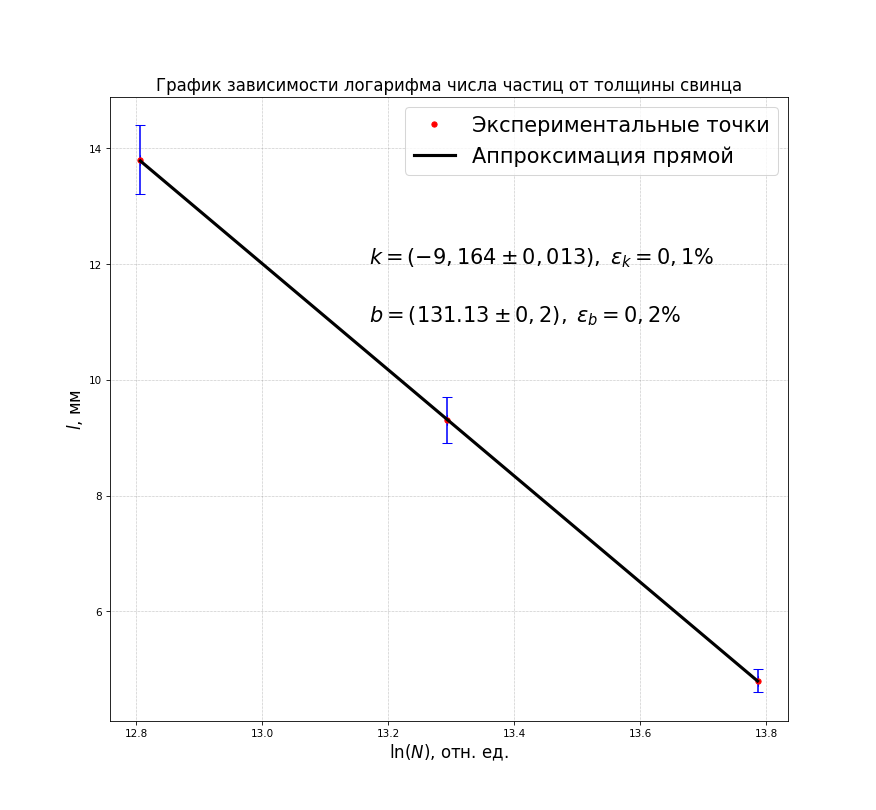
\includegraphics[width = \textwidth]{l(lnN)Pb.png}
\end{figure}

\[\mu = -\frac{1}{k} \approx 1,09 \text{ см}^{-1},\; \varepsilon_\mu = \varepsilon_k \approx 0,1\%\]

\newpage
\begin{figure}[H]\label{fig: l(lnN)Al}
    \centering
    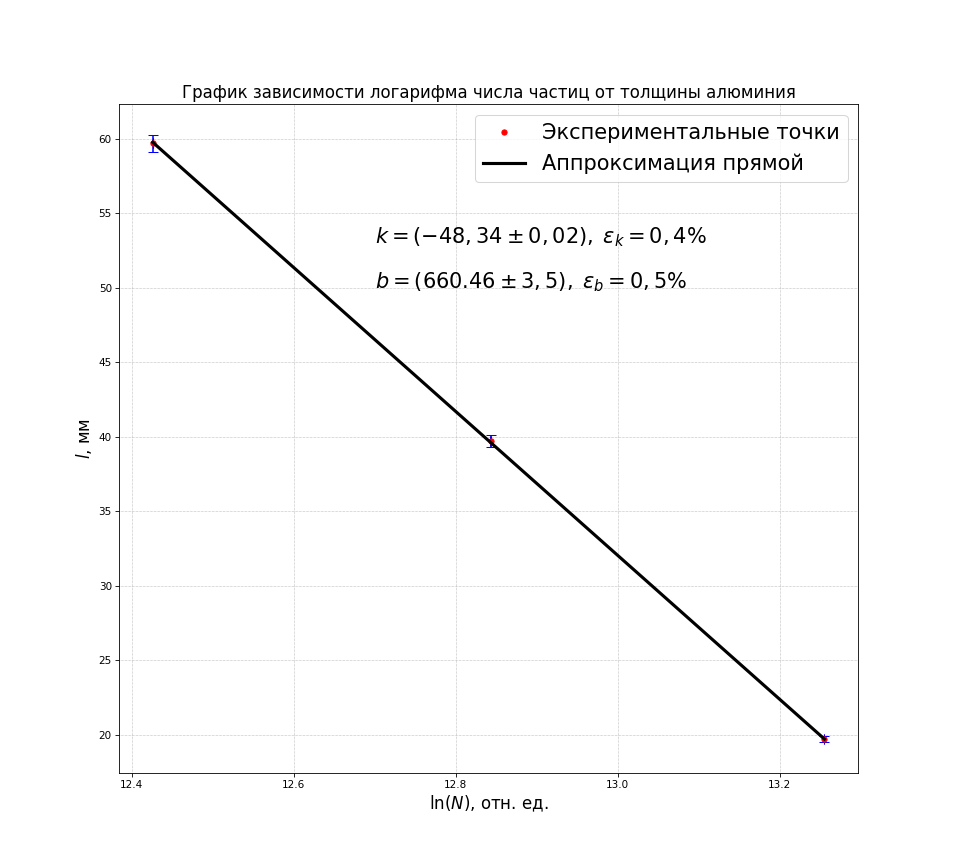
\includegraphics[width = \textwidth]{l(lnN)Al.png}
\end{figure}

\[\mu = -\frac{1}{k} \approx 0,21 \text{ см}^{-1},\; \varepsilon_\mu = \varepsilon_k \approx 0,4\%\]

\newpage
\begin{figure}[H]\label{fig: l(lnN)Fe}
    \centering
    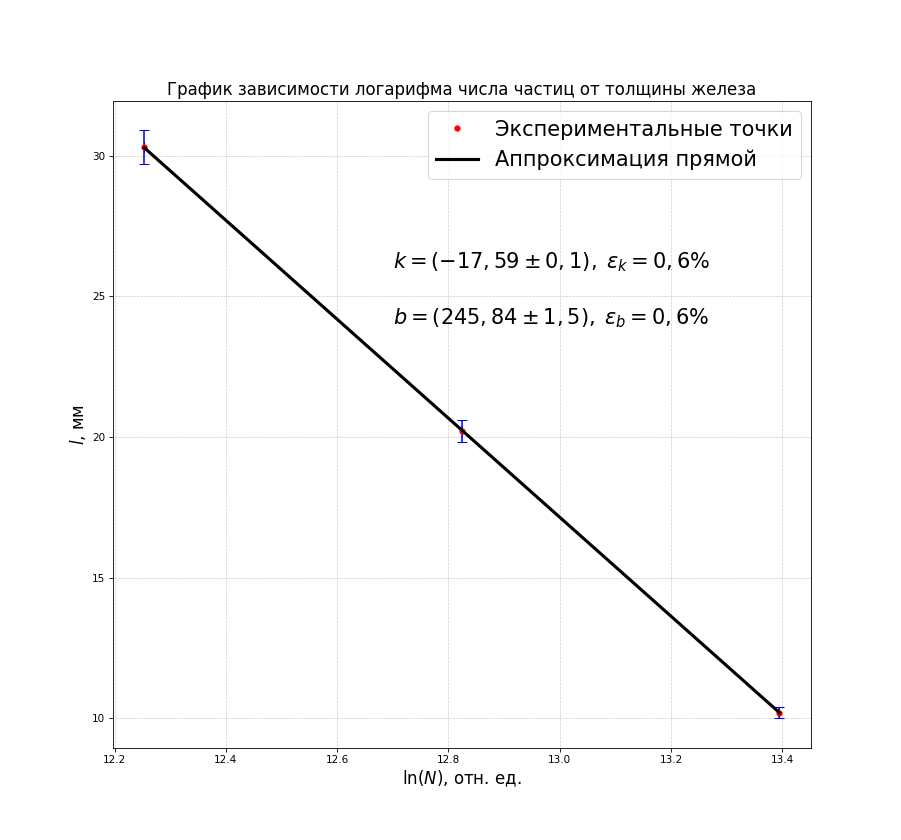
\includegraphics[width = \textwidth]{l(lnN)Fe.png}
\end{figure}

\[\mu = -\frac{1}{k} \approx 0,57 \text{ см}^{-1},\; \varepsilon_\mu = \varepsilon_k \approx 0,6\%\]
%%%%%%%%%%%%%%%%%%%%%%%%%
\end{document}
